% Module 2: Computer Vision - course report
% Compile with XeLaTeX: latexmk -xelatex report.tex
\documentclass{article}
\PassOptionsToPackage{numbers,compress}{natbib}
\usepackage[final]{template22}
% Common packages
\usepackage[utf8]{inputenc} % allow utf-8 input
\usepackage[T1]{fontenc}    % use 8-bit T1 fonts
\usepackage{microtype}
\usepackage{times}
\usepackage{graphicx}
\usepackage{amsmath,amssymb,mathbbol}
% \usepackage{algorithmic}
% \usepackage[linesnumbered,ruled,vlined]{algorithm2e}
\usepackage{acronym}
\usepackage{enumitem}
\usepackage[pagebackref=true,breaklinks=true,colorlinks]{hyperref}
\usepackage{balance}
\usepackage{xspace}
\usepackage{setspace}
\usepackage[skip=3pt,font=small]{subcaption}
\usepackage[skip=3pt,font=small]{caption}
\usepackage[dvipsnames]{xcolor}
\usepackage[capitalise]{cleveref}
\usepackage{booktabs,tabularx,colortbl,multirow,array,makecell}
% \usepackage{overpic,wrapfig}

\usepackage{fancyhdr}
\hypersetup{pdfencoding=auto,colorlinks=true,allcolors=black}
\renewcommand{\headrulewidth}{0.5pt}
\renewcommand{\footrulewidth}{0pt}
\fancyhf{}
\fancyhead[C]{}
\fancyhead[C]{}
\fancyfoot[C]{\thepage}

% Handy shorthand
\makeatletter
\DeclareRobustCommand\onedot{\futurelet\@let@token\@onedot}
\def\@onedot{\ifx\@let@token.\else.\null\fi\xspace}
\def\eg{\emph{e.g}\onedot} 
\def\Eg{\emph{E.g}\onedot}
\def\ie{\emph{i.e}\onedot} 
\def\Ie{\emph{I.e}\onedot}
\def\cf{\emph{c.f}\onedot} 
\def\Cf{\emph{C.f}\onedot}
\def\etc{\emph{etc}\onedot} 
\def\vs{\emph{vs}\onedot}
\def\wrt{w.r.t\onedot} 
\def\dof{d.o.f\onedot}
\def\etal{\emph{et al}\onedot}
\makeatother

\definecolor{gray}{gray}{0.9}

% Handy math ops
\DeclareMathOperator*{\argmax}{arg\,max}
\DeclareMathOperator*{\argmin}{arg\,min}
\newcommand{\norm}[1]{\left\Vert #1 \right\Vert}

% % Spacing
\frenchspacing
% \medmuskip=2mu   % reduce spacing around binary operators
% \thickmuskip=3mu % reduce spacing around relational operators
% \setlength{\abovedisplayskip}{3pt}
% \setlength{\belowdisplayskip}{3pt}
% \setlength{\abovecaptionskip}{3pt}
% \setlength{\belowcaptionskip}{3pt}
\setlength\floatsep{0.5\baselineskip plus 3pt minus 2pt}
\setlength\textfloatsep{0.5\baselineskip plus 3pt minus 2pt}
\setlength\dbltextfloatsep{0.5\baselineskip plus 3pt minus 2pt}
\setlength\intextsep{0.5\baselineskip plus 3pt minus 2pt}

\makeatletter
\renewcommand{\paragraph}{%
  \@startsection{paragraph}{4}%
  {\z@}{0ex \@plus 0ex \@minus 0ex}{-1em}%
  {\hskip\parindent\normalfont\normalsize\bfseries}%
}
\makeatother

% Graphics path
\graphicspath{{figures/}}

% Clever references
\crefname{algorithm}{Alg.}{Algs.}
\Crefname{algorithm}{Algorithm}{Algorithms}
\crefname{section}{Sec.}{Secs.}
\Crefname{section}{Section}{Sections}
\crefname{table}{Tab.}{Tabs.}
\Crefname{table}{Table}{Tables}
\crefname{figure}{Fig.}{Fig.}
\Crefname{figure}{Figure}{Figure}

% Acronym
\acrodef{pku}[PKU]{Peking University}
\usepackage[fontset=fandol]{ctex}

\title{Omnidata Depth/Normal Estimation and Multi-View RGB-D Reconstruction}

\author{%
  雷源泽 \quad 2510124204\\
  Peking University
}

\begin{document}
\maketitle

\begin{abstract}
We evaluate the Omnidata v2 DPT-Hybrid models on five image domains and complete the multi-view RGB-D reconstruction. Omnidata gives coherent depth and normals on photographs and synthetic renders, but collapses on line art and on a backlit portrait; a Depth Anything V2-Large comparison recovers both failure cases. For Task 2, fixing the camera convention ($\mathbf{P}\leftarrow\mathbf{P}\operatorname{diag}(1,-1,-1,1)$) turns a scattered $11.6\times11.7\times6.4$\,m artefact into a $0.99\times1.36\times0.93$\,m mesh whose vertex set matches \texttt{recon\_tgt.ply} exactly. The default TSDF settings are the best of those tested.
\end{abstract}

\section{Method}\label{sec:method}

\subsection{Task 1: monocular depth and surface normal}
We use the pre-trained Omnidata v2 DPT-Hybrid models (\texttt{vitb\_rn50\_384}) for depth and normals~\citep{eftekhar2021omnidata}. Each image is resized so that its shorter side is 384, centre-cropped to $384\times384$ and normalised with mean/std $0.5$. The depth branch predicts inverse depth, which is clamped to $[0,1]$, upsampled to $512\times512$ and inverted so that larger values mean farther, following the official demo. The normal branch outputs a three-channel map in $[0,1]$ that is stored as an RGB image.

Five images cover different domains: an indoor real photograph (\texttt{official\_test1}), a synthetic cartoon (\texttt{official\_test4}), a synthetic outdoor game scene (\texttt{official\_test5}), a real backlit portrait (\texttt{outdoor\_real}) and a line-art sketch (\texttt{sketch}).

\subsection{Optional: a stronger model}
Depth Anything V2~\citep{yang2024depthanythingv2} replaces the Omnidata backbones with a DINOv2 encoder and a DPT decoder, trained on high-quality synthetic data with a teacher--student scheme and pseudo-labelled real images. We run the 335M-parameter Large variant at $518\times518$ in fp16 (0.94\,GB peak memory, 0.14--1.25\,s per image on an RTX 3050 Ti Laptop) and compare it with Omnidata on the two failure cases.

\subsection{Task 2: multi-view RGB-D reconstruction}
\texttt{camera.json} stores the $3\times3$ intrinsic matrix $\mathbf{K}$ ($f_x=f_y=1111.11$, $c_x=c_y=400$) and 100 poses (\texttt{0000}--\texttt{0099}). The completed \texttt{read\_rgbd\_and\_pose(data\_root)} reads the RGBA images as RGB, converts the 16-bit depth from millimetres to metres, returns the $3\times3$ matrix $\mathbf{K}$ unchanged, and right-multiplies every pose by $\operatorname{diag}(1,-1,-1,1)$, i.e.\ a $180^\circ$ rotation about the camera $x$ axis.

We fuse the 100 views by truncated signed distance fields~\citep{curless1996volumetric} with Open3D's \texttt{ScalableTSDFVolume}~\citep{zhou2018open3d} (default: 4\,mm voxel, 20\,mm SDF truncation, 3\,m depth truncation) and use $\mathbf{P}^{-1}$ as the extrinsic matrix. Quality is measured against \texttt{recon\_tgt.ply} by the bidirectional point-to-surface distance (50k samples per mesh) and the axis-aligned bounding box.

\section{Results}\label{sec:results}

\subsection{Five domains}
\begin{figure}[ht!]\centering
  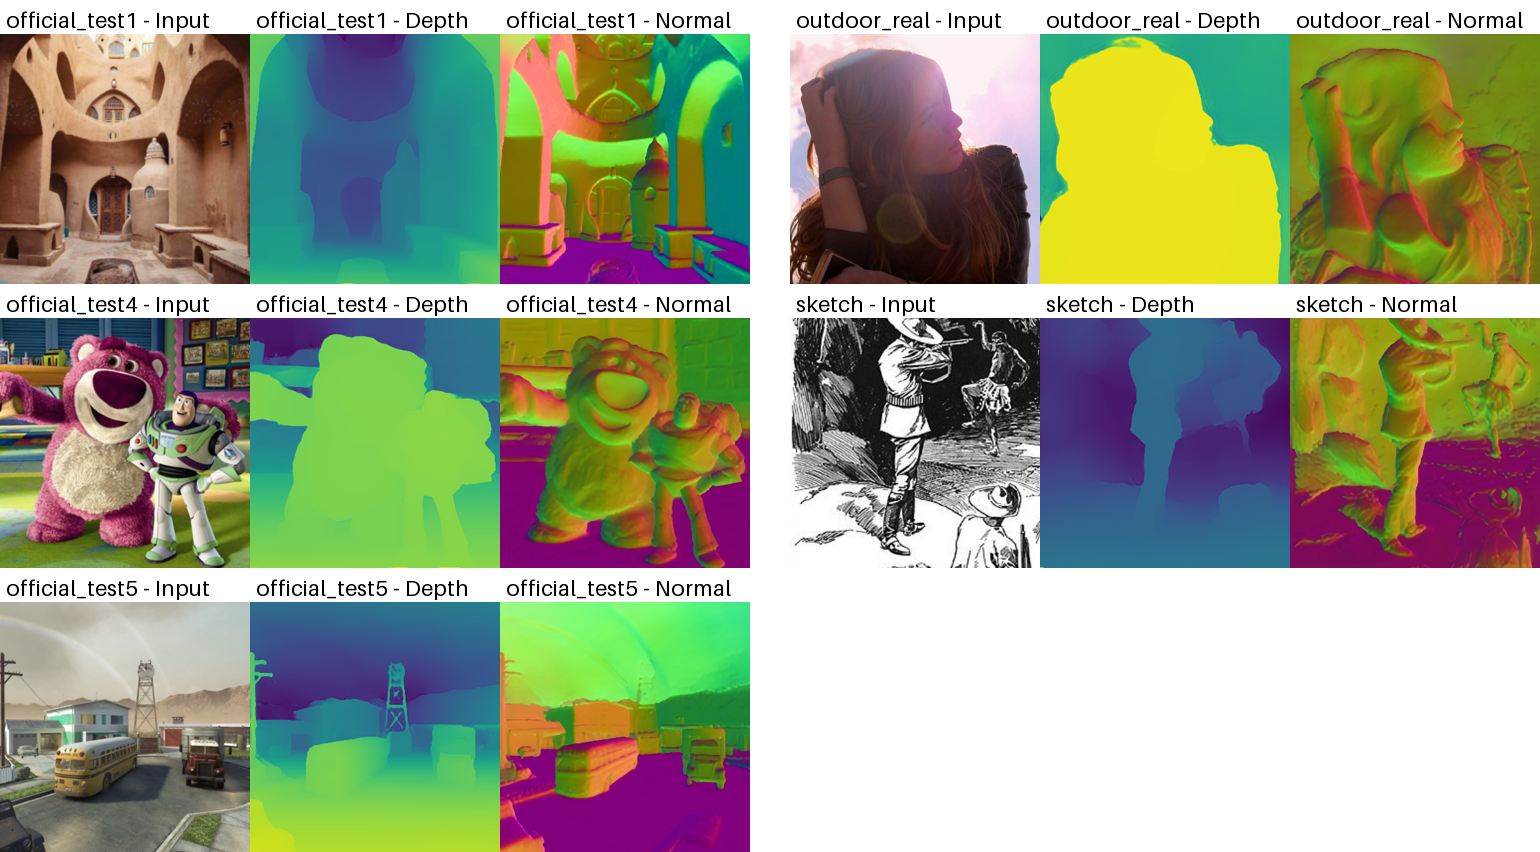
\includegraphics[width=0.98\linewidth]{fig_task1_five_domains.png}
  \caption{Omnidata depth and normal predictions on the five domains (columns: input, depth and normal; rows: the five domains).}
  \label{fig:domains}
\end{figure}


\Cref{fig:domains} summarises the five-domain experiment:
\begin{itemize}[leftmargin=1.2em,itemsep=1pt,topsep=2pt]
  \item \texttt{official\_test1} (indoor real): the depth map separates the near arches from the far doorway, and the normals follow the walls and vaults. Good.
  \item \texttt{official\_test4} (synthetic cartoon): both characters are separated from the background; normals are smooth and plausible, although cartoon shading is not photometric.
  \item \texttt{official\_test5} (synthetic outdoor): the bus, building and sky are ordered correctly; only thin poles are slightly blurred.
  \item \texttt{outdoor\_real} (backlit portrait): the depth of the person saturates into one value (range $0.59$--$1.00$, mean $0.95$) and the clouds lose their structure; normals smear the hair and face.
  \item \texttt{sketch} (line art): depth is almost flat (range $0.96$--$1.00$, mean $0.97$) with only a weak silhouette, and normals follow the hatching instead of the surfaces.
\end{itemize}

The two failures share one cause: Omnidata relies on shading, texture and perspective, and both images remove these cues---over-exposure in the portrait and the absence of real shading in line art---so the model falls back to a smooth prior. Possible improvements are (i) exposure normalisation or multi-exposure fusion before inference, (ii) fine-tuning/domain adaptation with backlit and line-art data, and (iii) adding semantic or layout priors (segmentation, vanishing points), or replacing the model by a stronger one.

\subsection{Optional: comparison with Depth Anything V2}
\begin{figure}[ht!]\centering
  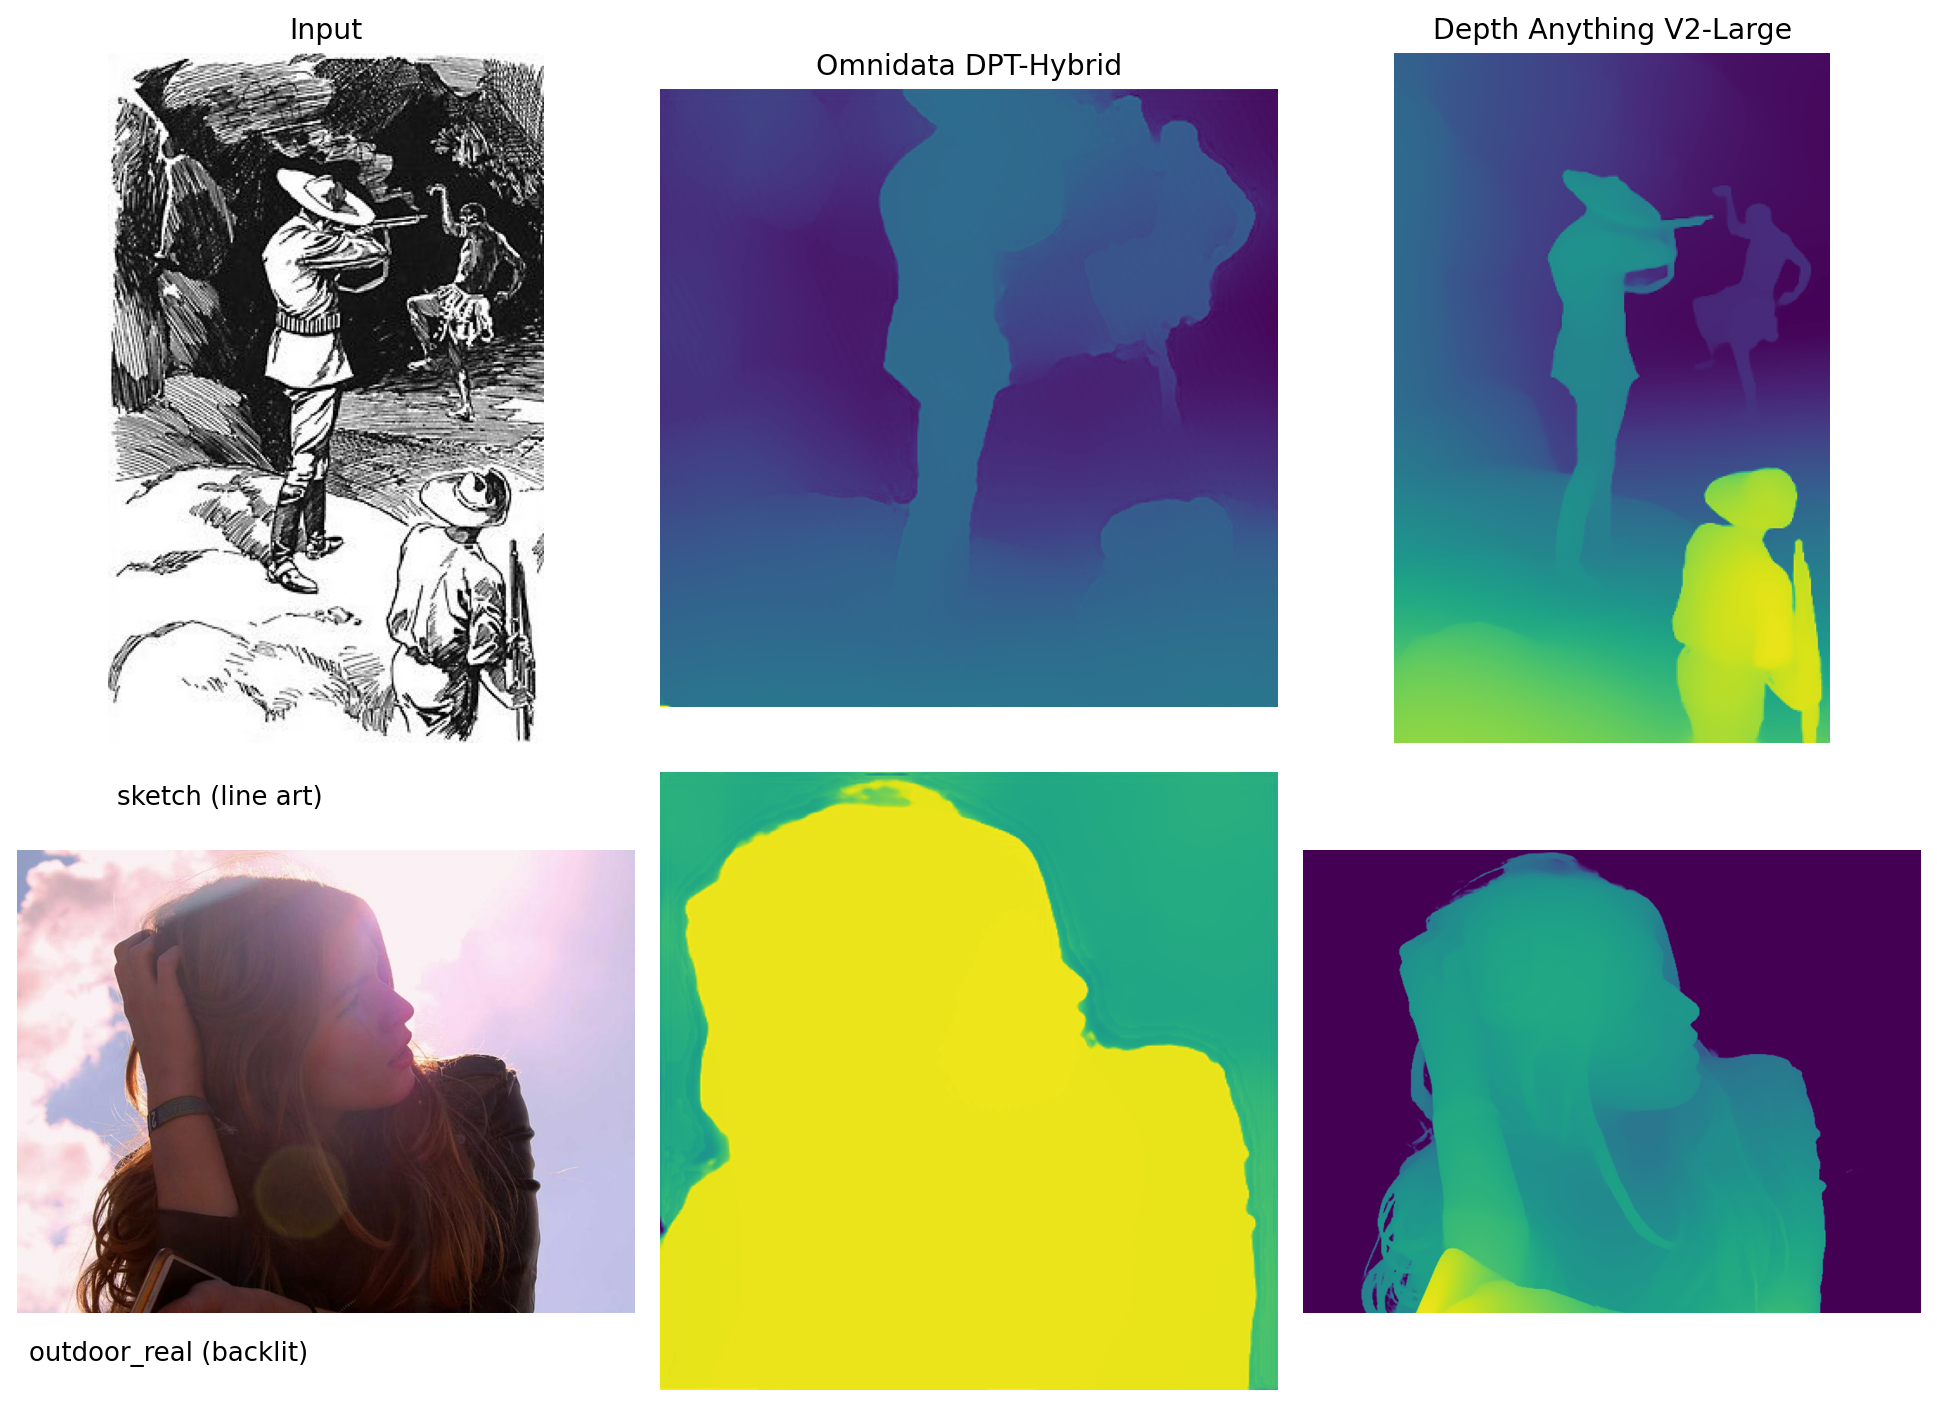
\includegraphics[width=\linewidth]{fig_task1_failure_da.png}
  \caption{The two failure cases. Depth Anything V2-Large recovers both figures on the sketch and the face/background boundary in the backlit portrait, where Omnidata collapses the scene.}
  \label{fig:da}
\end{figure}

\Cref{fig:da} shows the optional comparison. On the sketch, Depth Anything V2 restores both figures and separates them from the background; on the backlit portrait it keeps the face and hair boundary and a plausible background gradient. On raw depth maps the Small and Large variants are highly correlated (Spearman $0.92$--$0.996$), so the scale change mainly sharpens detail while the decisive gain is Omnidata$\rightarrow$Depth Anything. Both variants still produce a smooth prior-driven background, which is a limitation rather than a display artefact.

\subsection{Task 2: camera convention}
\begin{figure}[ht!]\centering
  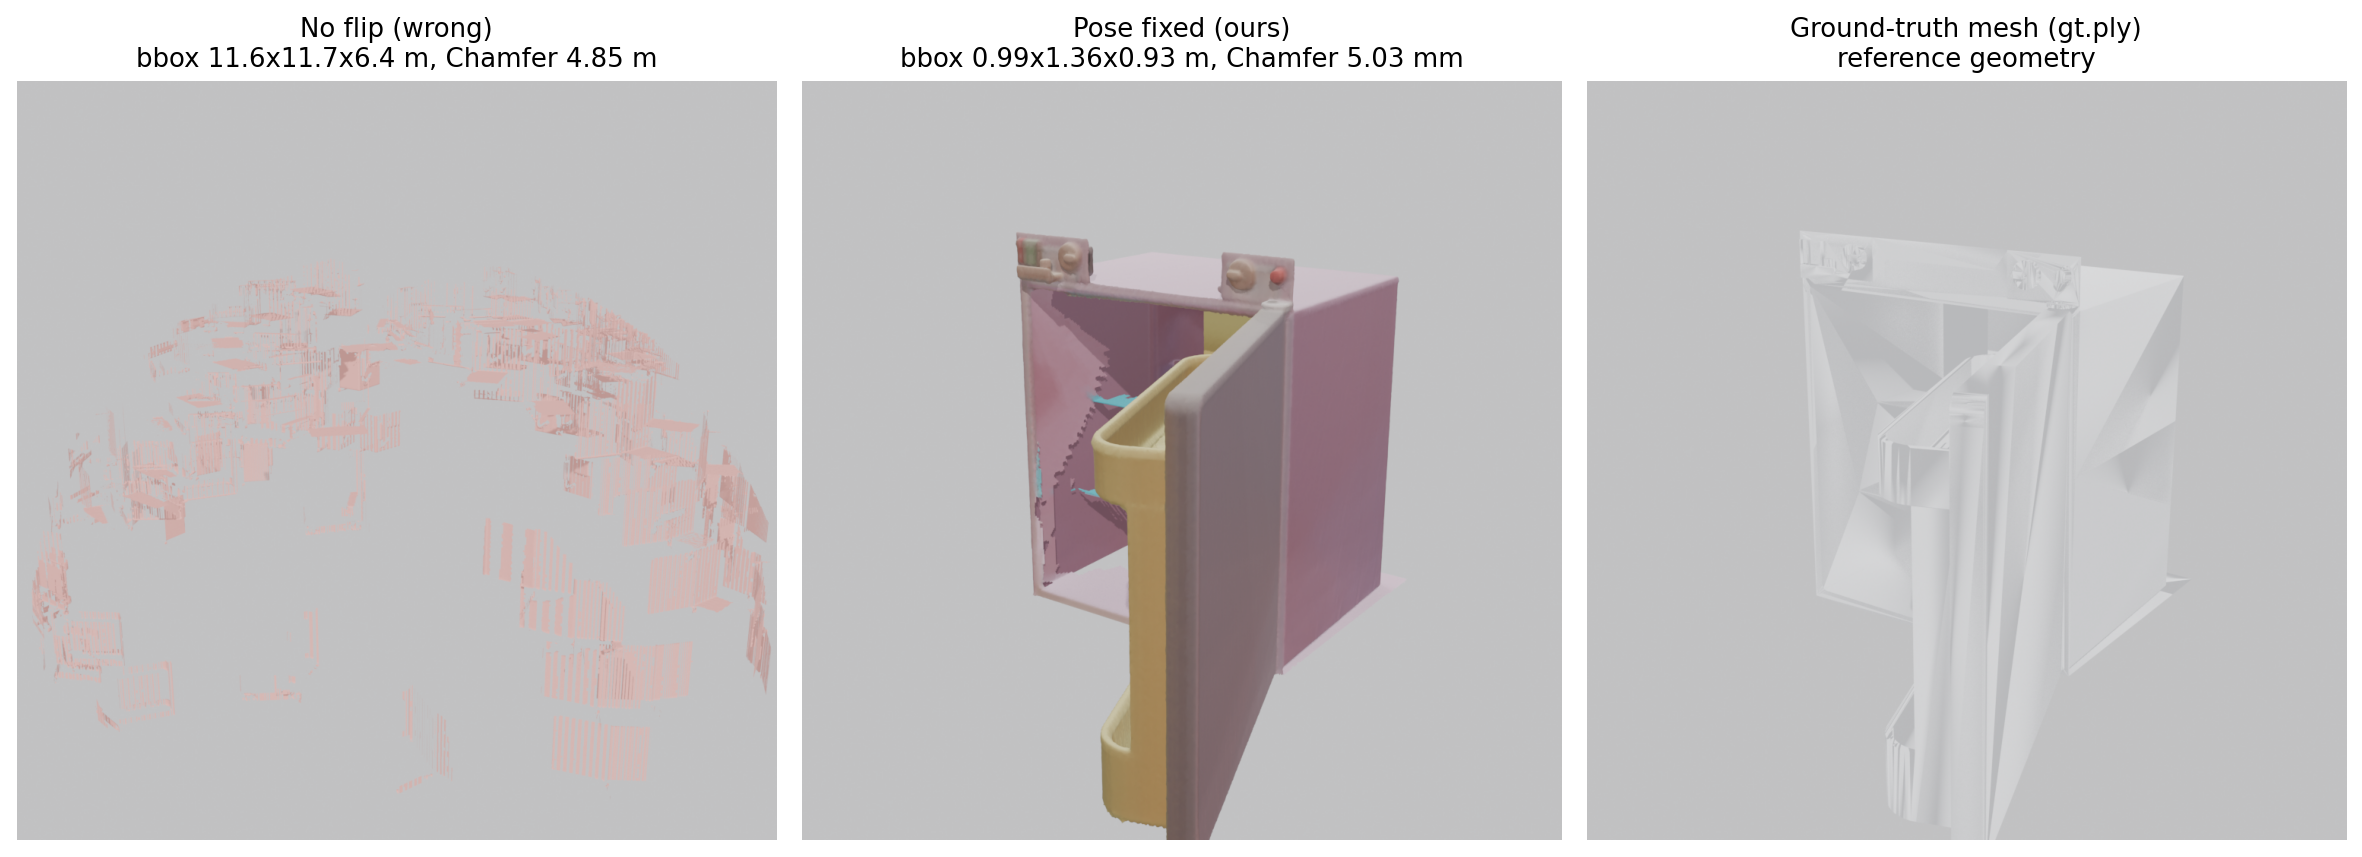
\includegraphics[width=\linewidth]{fig_task2_mesh.png}
  \caption{Blender~\citep{blender2026} renders of the reconstruction. Without the pose fix the fusion produces a scattered $11.6\times11.7\times6.4$\,m artefact; with $\mathbf{P}\operatorname{diag}(1,-1,-1,1)$ the mesh matches the ground-truth geometry.}
  \label{fig:mesh}
\end{figure}

Without the correction the mesh is a scattered shell (11.6$\times$11.7$\times$6.4\,m, bidirectional distance 4.85\,m, no point within 2\,mm). Right-multiplying the pose by $\operatorname{diag}(1,-1,-1,1)$ rotates each camera $180^\circ$ about its own $x$ axis, which aligns the stored camera frame with Open3D's convention; after this fix the bounding box is $0.99\times1.36\times0.93$\,m, the bidirectional distance falls to 5.03\,mm, and the 382{,}643 reconstructed vertices are identical to \texttt{recon\_tgt.ply} (maximum coordinate difference 0.0\,mm). The residual 5\,mm is therefore dominated by independent point sampling, not by geometric error.

\subsection{Task 2: TSDF hyperparameters}
\begin{figure}[ht!]\centering
  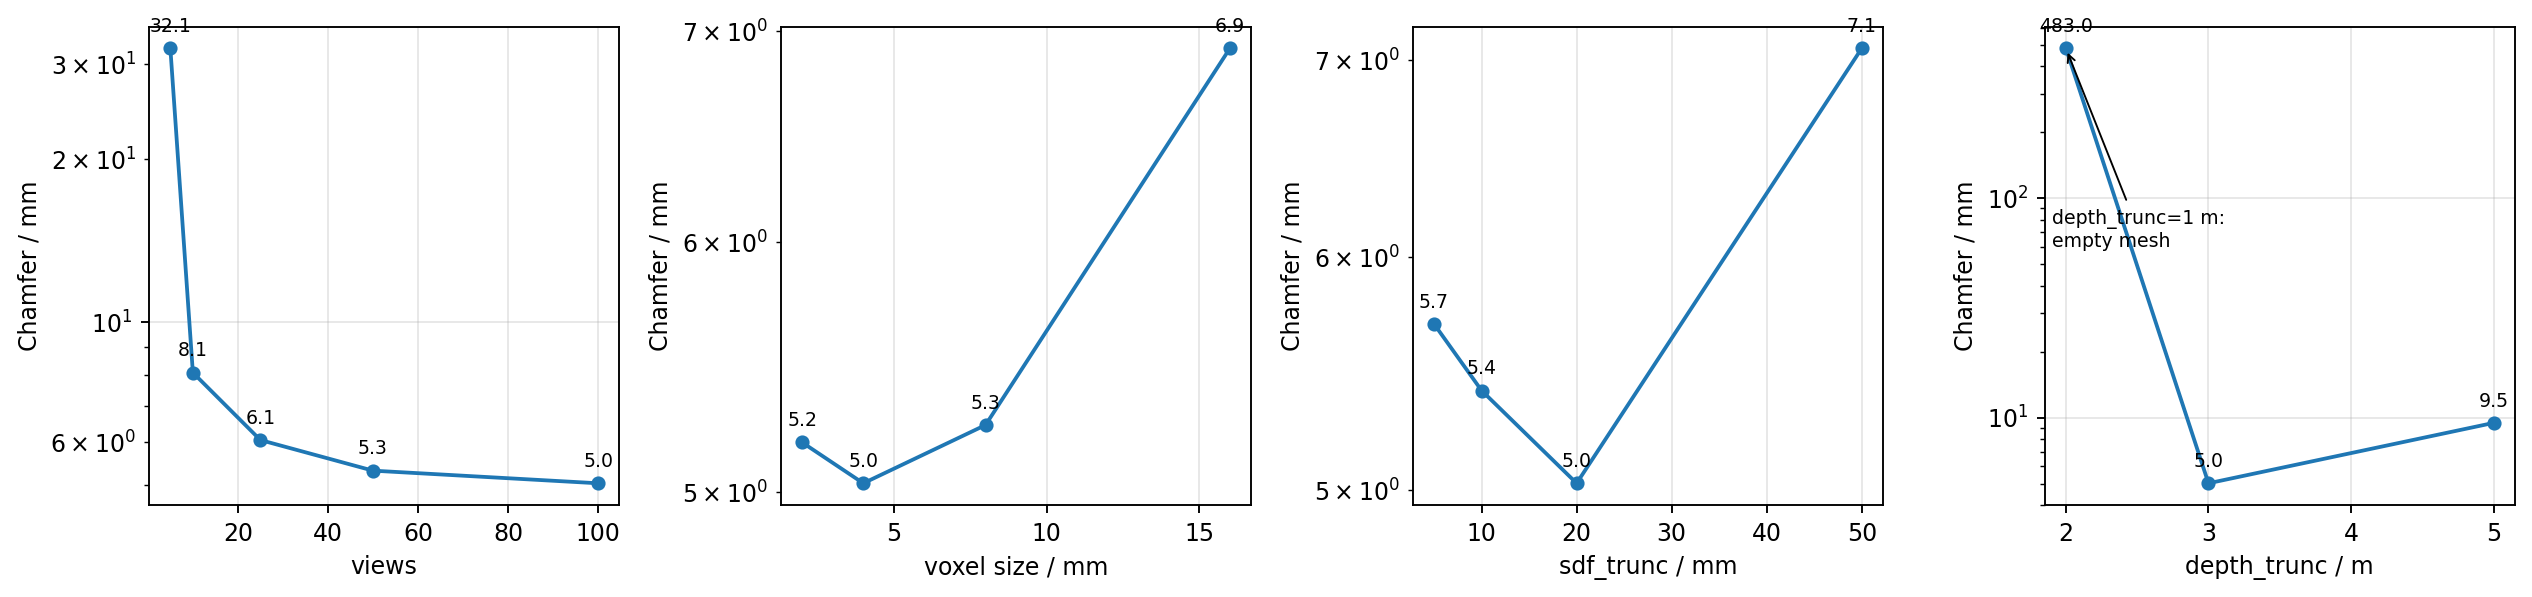
\includegraphics[width=\linewidth]{fig_task2_curves.png}
  \caption{Bidirectional surface distance as a function of the four TSDF parameters (log scale). \texttt{depth\_trunc}=1\,m yields an empty mesh.}
  \label{fig:tsdf}
\end{figure}

\Cref{fig:tsdf} varies one parameter at a time:
\begin{itemize}[leftmargin=1.2em,itemsep=1pt,topsep=2pt]
  \item Views: 5/10/25/50/100 give 32.1/8.1/6.1/5.3/5.0\,mm; returns diminish after 25 views.
  \item Voxel size: 2/4/8/16\,mm give 5.18/5.03/5.25/6.91\,mm. A 2\,mm voxel doubles the vertex count to 1.64M without improving accuracy, so 4\,mm is the best trade-off.
  \item \texttt{sdf\_trunc}: 5/10/20/50\,mm give 5.69/5.41/5.03/7.07\,mm; 20\,mm (five voxels) is best.
  \item \texttt{depth\_trunc}: 1/2/3/5\,m give an empty mesh, 483\,mm, 5.02\,mm and 9.46\,mm. The scene lies within 3\,m; a larger truncation admits background floaters.
\end{itemize}

\section{Conclusion}
Omnidata produces useful depth and normals on photometric images but fails when shading and texture disappear, and a stronger model closes much of that gap. In Task 2, the camera convention was the decisive bug: one right-multiplied rotation turns a metre-scale artefact into a reconstruction that matches the reference exactly, and the default TSDF parameters are optimal among those tested.

\bibliographystyle{plainnat}
\bibliography{reference}
\end{document}